\documentclass{article}
%\usepackage{authblk}

\usepackage{graphicx}
\usepackage{float}
%\usepackage{fullpage}
\usepackage[utf8]{inputenc}
\usepackage{hyperref}

\usepackage[spanish]{babel}
\usepackage{amssymb,amsmath}
\usepackage{caption}
\captionsetup[figure]{font=scriptsize,labelfont=scriptsize}
\decimalpoint

%\usepackage[backend=bibtex,
%style=authoryear
%style=alphabetic
%style=reading
%]{biblatex}
%\addbibresource{bib}

\usepackage{xcolor}


\title{Algoritmos de deformación de mallas poligonales para sistemas de 
procesamiento digital de geometría}

\author{Plan de Tesis\\
        Director: Gabriel Taubin\\
        Co-director: Fernando Cukierman\\
        Consejero de estudios: Agustín Gravano\\
        Estudiante: Manuel Dubinsky}


\begin{document}


% Doctorado UBA: Artículo 10º. El tema y Plan de Tesis deberán ser presentados a la Comisión de Doctorado para su consideración y eventual aprobación por el Consejo Directivo, con el consentimiento del Director de Trabajo de Investigación y Plan de Tesis propuesto y del codirector, si lo hubiere, y una explicación de éste/os acerca de los medios disponibles para ser realizado, indicando el lugar donde se llevará a cabo la investigación. El Trabajo de Tesis deberá ser inédito y original. La publicación parcial de sus resultados con la aprobación del Director de Trabajo de Investigación y Plan de Tesis no invalidará el carácter de inédito requerido.

% Doctorado exactas: ARTICULO 14.-
% 14.1. Dentro de los dos (2) años de la aprobación del examen de admisión el Director de Tesis presentará el Plan de Tesis para su consideración a la Comisión de Doctorado, conjuntamente con el Doctorando. El mismo deberá contener la siguiente información:
% a- El tema de investigación sobre el cual versará el trabajo de Tesis.
% b- Lugar de trabajo.
% c- Antecedentes existentes sobre el tema.
% d- Naturaleza del aporte original proyectado.
% e- Disponibilidad de infraestructura y factibilidad de desarrollo del trabajo y su financiamiento.
% f - Plan de Trabajo.

\maketitle

%\begin{abstract}
%TODO
%\end{abstract}

%\tableofcontents

%\newpage

\section{Tema de investigación}
En los últimos años se ha producido una revolución técnica que generó un 
crecimiento sin precedentes en la capacidad de procesamiento de datos de 
los dispositivos de uso personal (ej.: notebooks y teléfonos celulares). 
En sintonía con esos cambios, el paradigma global en torno a la creación de 
software libre ha puesto a disposición herramientas sofisticadas de 
excelente calidad. En particular han surgido muchas herramientas de diseño 
para la industria, la arquitectura y el urbanismo, la exploración geográfica y 
el entretenimiento (ej.: cine de animación y juegos). Por otro 
lado, actualmente es posible producir modelos digitales 
tridimensionales muy precisos tomados de la realidad en base a diversas 
técnicas: resonancia magnética, tomografía computarizada, láser, 
ultrasonido, radarización, microscopía, etc. A las cuales se suman técnicas 
más económicas basadas en procesamiento de imágenes. 
Por último, hoy en día es posible producir objetos tridimensionales de 
buena calidad y bajo costo en base a técnicas de impresión 3D. La conjunción 
de estos tres hechos en relación al modelado tridimensional: (1) sistemas de 
captura de datos, (2) software de procesamiento e (3) impresión 3D, están determinando 
cambios drásticos en la producción de bienes y servicios.

% buscar alguna referencia de digital fabrication
\

El área de Procesamiento Digital de Geometría es la rama de la Ciencia 
de la Computación encargada de elaborar los modelos y algoritmos para 
analizar y manipular la información geométrica de los objetos 
tridimensionales. Más precisamente, provee herramientas para: reconstruir 
superficies a partir de conjuntos de puntos, filtrar el ruido en las 
muestras de puntos y manipular las formas (ej.: simplificarlas, deformarlas,
 suavizarlas y parametrizarlas) \cite{BKPAL:2010}. Se encarga además de 
 formular las estructuras de datos para modelar la información geométrica. 
 En este sentido, las mallas poligonales son las representaciones discretas 
 de los  objetos. Básicamente son grafos \cite{Harari:1969} que modelan 
 superficies inmersas en el espacio tridimensional. Sus vértices son  
 una muestra de los puntos de la superficie. A cada vértice de la 
 malla se le asocia su posición en el espacio (ej.: coordenadas cartesianas). 
 Los ciclos simples del grafo se denominan “caras”. Las caras son polígonos 
 convexos simples (en general triángulos o cuadrados) que modelan una pequeña 
 parte de la superficie aproximando linealmente sus puntos interiores.

\

El contexto de nuestro trabajo es el problema de \emph{deformación de mallas 
poligonales}. Específicamente, una deformación $d: S \rightarrow S'$ es un 
mapa de una superficie $S$ en otra $S'$ que asocia a cada punto $p \in S$ 
un vector de desplazamiento $d(p)$, de este modo la superficie $S$ es 
deformada en la superficie $S'$:

$$S' := \{p + d(p) \ | \ p \in S\}$$

Para una representación de la superficie en términos de una malla poligonal, 
una deformación está completamente determinada por los vectores de desplazamiento 
$d_i = d(p_i)$ de los vértices de la malla $p_i \in S$. De modo que los 
desplazamientos de los puntos interiores de las caras se aproximan linealmente.

\

En la práctica, este problema debe ser considerado en el contexto de enriquecer 
la funcionalidad de las herramientas de diseño tridimensional. Es decir, por 
un lado hay que proveerle a los usuarios una interface simple para definir 
deformaciones de las superficies y por el otro, los algoritmos deben ser eficientes 
para brindar una respuesta interactiva. Típicamente la interface con los 
usuarios consiste en permitirles definir dos regiones sobre la superficie: 
(1) una región $H$ denominada \emph{manija} y una transformación afín (desplazamiento 
y/o rotación) de $H$ y (2) una región fija $F$ que permanecerá invariante. 
El algoritmo de deformación se encargará de producir una transformación 
suave del conjunto de puntos intermedios entre $F$ y $H$ (figura \ref{fig:def}). 
Denotaremos $R$ a dicho conjunto de puntos intermedios.

\

Nuestro trabajo consiste en diseñar e implementar nuevos algoritmos de 
deformación de superficies que resulten prácticos para las herramientas 
de diseño e impresión 3D.

\begin{figure}
	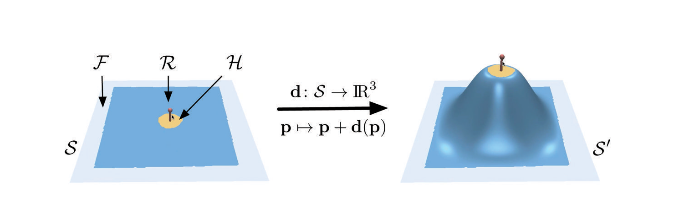
\includegraphics[scale=.5]{deformacion.png} % Figure image
	\caption{Una deformación $d: S \rightarrow S'$. Se define la manija 
	$H$ (región amarilla) y se desplaza verticalmente. La región 
	fija $F$ (gris) permanece invariante. La región $R$ (azul) entre $F$ 
	y $H$ se deforma suavemente.}% Figure caption
	\label{fig:def} % Label for referencing with \ref{bear}
\end{figure}

\section{Antecedentes existentes sobre el tema}

Esencialmente hay dos grandes enfoques para abordar el problema 
de deformación de mallas poligonales: (1) deformaciones intrínsecas de la 
superficie y (2) deformaciones del espacio. Por un lado, las deformaciones 
intrínsecas consideran que la 
función de desplazamientos $d: S \rightarrow \mathbb{R}^3$ se define sobre 
la superficie $S$ y se calcula a partir de su malla poligonal asociada. Los 
métodos derivados de este enfoque son muy flexibles porque las condiciones 
se definen sobre cada vértice de la malla. Esa definición local de las 
condiciones incrementa los grados de libertad de las deformaciones. El inconveniente 
que presentan estas técnicas es que su eficiencia y robustez está asociada 
a la complejidad de la superficie y a la calidad de la muestra de puntos 
que conforman la malla poligonal. Por otro lado, el enfoque mediante deformaciones 
del espacio, considera que la función de desplazamientos $d: \mathbb{R}^3 
\rightarrow \mathbb{R}^3$ aplica sobre el espacio ambiente en el que está 
inmersa la superficie. De modo tal que la superficie se deforma implícitamente 
de acuerdo a la deformación global del espacio que la contiene. \\
A continuación presentamos los métodos más conocidos de cada uno de los  
enfoques. Recordemos de la sección anterior los tres conjuntos que intervienen 
en una deformación: (1) el conjunto $H$ (manija), (2) el conjunto $F$ (conjunto 
fijo o invariante) y (3) el conjunto $R$ (conjunto de puntos intermedios, 
o sea el soporte de la deformación).

\subsection{Métodos de deformaciones intrínsecas de la superficie}
Dentro de este enfoque, las técnicas más simples denominandas \emph{técnicas 
de propagación} consisten en propagar la transformación afín de la manija 
($H$) al conjunto $R$. Para que la transformación resulte suave entre $H$ 
y $F$, la propagación se regula mediante una función de distancia 
$s: R \rightarrow [0,1]$ de cada punto de $R$ al conjunto fijo ($F$). Dicha 
función permite controlar para cada punto la magnitud de la transformación, 
de modo tal que los puntos cercanos a $H$ se transformen en mayor proporción 
que los puntos cercanos a $F$. La función de distancia ($s$) puede estar 
asociada a una distancia geodésica sobre la superficie 
\cite{BK:2003} o a una distancia euclídea en el espacio ambiente \cite{P:2003}. 
Estas técnicas son simples pero las deformaciones que resultan de ellas 
pueden ser poco intuitivas en el sentido de que a veces no modelan efectos 
de fuerzas físicas actuando sobre la superficie.

\

La técnica \emph{shell-based} inspirada en modelos físicos produce deformaciones 
más intuitivas. Minimiza ciertas funciones de energía que modelan el estiramiento 
y la curvatura de la superficie. El modelo general involucra ciertas nociones 
geométricas; dada una superficie $S$ se definen $I$ y $II$, la primera y 
segunda forma fundamental \cite{doCarmo:1976}. Miden el área y la curvatura 
infinitesimal en cada entorno de la superficie. Por otro lado, una deformación 
de la superficie $S$ tiene asociadas sus propias formas fundamentales: $I'$ 
y $II'$. La idea es encontrar la deformación $S'$ que minimice la energía:

$$E(S') = \int \int ||I - I'||^2 + ||II-II'||^2$$

Informalmente, la minimización de la expresión está asociada a una deformación 
cuyo estiramiento y curvatura global requiere la mínima energía posible 
(en términos físicos) \cite{T:1987}. \\
Para poder aplicar el modelo general a una malla poligonal es preciso definir 
una versión discreta. Para eso previamente se simplifica el modelo sustituyendo 
las formas fundamentales por derivadas parciales de la función de desplazamientos 
$d: S \rightarrow \mathbb{R}^3$ \cite{WW:1992}:

$$E(d) = \int \int (||d_u||^2 + ||d_v||^2) + 
(||d_{uu}||^2 + 2 ||d_{uv}||^2 + ||d_{vv}||^2) \ du \ dv$$

El problema se reformula en términos de encontrar la función de 
desplazamientos que minimiza la expresión. Para resolverlo, hay 
que resolver la ecuación diferencial de \emph{Euler-Lagrange} asociada:

$$\Delta d + \Delta^2 d = 0$$

Donde $\Delta$ es el \emph{operador de Laplace} \cite{E:1998}. La versión 
discreta se reduce a resolver un sistema lineal de la 
forma: $(L + L^2) \bar d = \bar b$ donde $L$ es una \emph{matriz laplaciana} 
\cite{B:2013}, $\bar b$ son las condiciones de iniciales de la ecuacion diferencial 
y $\bar d$ es el vector de los desplazamientos de los vértices de la malla 
poligonal.

\

El problema que presenta la técnica \emph{shell-based} es que al simplificar 
la formulacion del problema para transformarlo en un problema lineal, las 
deformaciones pueden perder calidad de los detalles de la superficie. Una 
forma de preservar esos detalles es complementarla con la técnica de deformacion 
\emph{multi-escala}. Esta técnica se inspira en nociones de procesamiento 
de señales. Consiste en descomponer a la superficie en dos (o más) bandas 
de frecuencias, de modo tal que la banda de frecuencias bajas corresponde 
a una version global suavizada (sin detalles) de la superficie y la banda 
de frecuencias altas corresponde a los detalles locales de la superficie. 
De este modo la deformacion se aplica sobre la banda de frecuencias bajas 
y a la superficie resultante se le agregan los detalles de la banda de 
frecuencias altas. Hay distintas variantes en relacion al tratamiento 
de los detalles, considerarlos como: vectores de desplazamientos \cite{K:1998}, 
desplazamientos respecto al vector normal \cite{K:1999}, desplazamientos de 
volúmenes \cite{BK:2003b}, transferencia de la deformacion a los detalles 
\cite{B:2006}.

\

Otro conjunto denominado \emph{técnicas diferenciales} consideran modificar 
propiedades diferenciales en lugar de coordenadas espaciales. Los dos ejemplos 
más conocidos consideran el \emph{gradiente} y el \emph{laplaciano}. Los 
métodos basados en el gradiente, modifican 
los gradientes de la superficie original y calculan la deformacion como  
aquella que minimiza (en términos de cuadrados mínimos) la diferencia respecto 
a los gradientes modificados (\cite{Y:2004}, \cite{Z:2005}). Los métodos 
basados en el \emph{laplaciano} son análogos (\cite{L:2004}, \cite{S:2004}, 
\cite{ZH:2005}). En ambos casos, la version discreta de estas técnicas implica 
resolver un sistema lineal laplaciano. 

\subsection{Métodos de deformaciones del espacio}
Las técnicas de \emph{deformaciones del espacio} deforman el espacio ambiente 
modificando implícitamente a la superficie. Es decir, consideran funciones 
de desplazamiento de la forma $d: \mathbb{R}^3 \rightarrow \mathbb{R}^3$.

\

La \emph{técnica de reticulado} parametriza el espacio ambiente 
mediante tres familias de \emph{B-splines} \cite{G:2015}:

$$f(u,v,w) = \sum_j \sum_k \sum_l c_{jkl} N_j(u) N_k(v) N_l(w)$$

Donde los $c_{jkl}$ son los puntos de control. En particular cada vértice de 
la superficie $f(u_i, v_i, w_i) = p_i \in S$ es una combinación lineal 
de estos:

$$p_i = f(u_i, v_i, w_i) = \sum_j \sum_k \sum_l c_{jkl} N_j(u_i) N_k(v_i) N_l(w_i)$$

Por otro lado, la deformación del espacio está especificada en términos 
de los desplazamiento de los puntos de control $\delta c_{jkl} = c_{jkl}' - c_{jkl}$:

$$d(u,v,w) = \sum_j \sum_k \sum_l \delta c_{jkl} N_j(u) N_k(v) N_l(w)$$

De manera que el desplazamiento del punto $p_i$ se calcula como $p_i' = 
p_i + d(u_i,v_i,w_i)$.

\

La \emph{técnica de encapsulamiento} es una generalización que en lugar 
de definir un reticulado de todo el espacio ambiente, considera una malla 
poligonal que encapsula a la superficie (figura \ref{fig:caballo}). Los 
puntos de la superficie se expresan como combinaciones lineales de los 
vértices de control definidos por la malla poligonal \cite{L:2008}. Y la 
deformación se implementa de modo análogo al procedimiento anterior.

\begin{figure}
	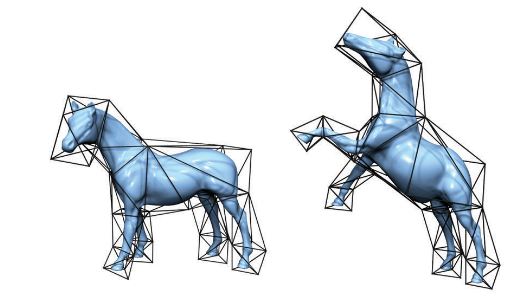
\includegraphics[scale=.5]{caballo.png} % Figure image
	\caption{\emph{Técnica de encapsulamiento}. Una malla poligonal 
	encapsula a la superficie y permite controlar su deformación.}% Figure caption
	\label{fig:caballo} % Label for referencing with \ref{bear}
\end{figure}

\subsection{Sistemas lineales}
El requerimiento de que las técnicas de deformación de superficies sean 
interactivas implica que los algoritmos deben ser eficientes. Este hecho 
se tradujo en una tendencia general de los autores a considerar versiones 
simplificadas del problema. Es decir que en general los métodos deben resolver 
 sistemas de ecuaciones lineales. Inclusive los sistemas lineales que surgen 
de las técnicas de deformación de mallas poligonales pertenecen a una clase 
más restringida: los sistemas laplacianos esparsos. Es decir que además 
la matriz es simétrica y definida positiva.

\

Los algoritmos de resolución de ecuaciones lineales se dividen en dos grupos: 
(1) \emph{métodos directos} y (2) \emph{métodos iterativos}. Los métodos 
directos producen una solución exacta y se basan en una factorización conveniente 
de la matriz. Los métodos iterativos son algoritmos de punto fijo en 
el sentido de que convergen monótonamente a la solución; estos métodos 
inducen una función que cuantifica el error en cada iteración 
$e^{(i)} = x^* - x^{(i)}$, donde $x^*$ es la solución exacta y $x^{(i)}$ 
es el valor calculado por el algoritmo en el $i$-esima iteración.

\

Algunos ejemplos de métodos directos consideran las siguientes factorizaciones 
de la  matriz ($M$): $M=LU$ (donde $L$ es triangular inferior y $U$ triangular 
superior), $M=QR$ (donde $Q$ es ortogonal y $R$ es triangular superior), 
descomposición en valores singulares ($M = U \Sigma V^*$, donde $U$ y $V^*$ 
son ortonormales y $\Sigma$ es diagonal) y $M = LL^t$ (donde $L$ es triangular 
inferior, esta descomposición es posible si $M$ es simétrica y definida 
positiva).

\

Por otro lado, los métodos iterativos más conocidos son: \emph{Jacobi}, 
\emph{Gauss-Seidel} y \emph{Gradiente Conjugado}. Son muy efectivos para 
atenuar las frecuencias altas del error $e^{(i)}$, pero se degrada mucho 
su eficiencia si el error es una función suave (como en el caso de los sistemas 
laplacianos). Por ese motivo se creó una variante denominada \emph{Multigrid}, 
que básicamente define un encaje de mallas poligonales de modo tal que 
los errores asociados a los sistemas lineales correspondientes definan 
funciones de menor suavidad para permitir mejorar la eficiencia.

\

También se crearon algunas variantes de los algoritmos directos específicamente 
para resolver sistemas esparsos. El más importante es el método de 
\emph{Cholesky Esparso}.

\

Del análisis de los algoritmos \cite{K:2005} surge que los métodos 
\emph{Multigrid} y \emph{Cholesky Esparso} son los más eficientes y 
permiten resolver sistemas lineales asociados a mallas de $10^5$ nodos 
de modo tal que pueden ser implementados por herramientas interactivas.

\

Finalmente, es importante mencionar que en el último tiempo ha
habido grandes avances en la creación de nuevos métodos
iterativos para resolver sistemas laplacianos (\cite{S:2010}, \cite{T:2010}, 
\cite{K:2010}). Estos métodos deberían ser considerados y adaptados en el 
contexto del área de Procesamiento Digital de Geometría.

\section{Naturaleza del aporte original proyectado}

Nuestro trabajo consiste en aportar nuevos enfoques al problema de 
deformación de mallas poligonales. Esto implica realizar aportes tanto en 
la creación de nuevos algoritmos como en la adaptación de los avances 
que se han producido en los últimos años en el área de resolución de 
sistemas lineales laplacianos a las técnicas ya existentes. Por otro lado, 
vamos a privilegiar realizar el trabajo en el marco de las herramientas 
\emph{open-source} de diseño e impresión 3D, porque entendemos que puede 
resultar de interés tanto a nivel académico como a nivel de la industria. 

\section{Lugar de trabajo, infraestructura, factibilidad de desarrollo del trabajo y su financiamiento}

El lugar de trabajo en el que se desarrolla mi doctorado es el Departamento 
de Tecnología y Administración de la Universidad Nacional de Avellaneda. 
Dicho trabajo no requiere una infraestructura que exceda las capacidades 
de una computadora personal, porque tanto el proceso de implementación como 
el de ejecución de los algoritmos tienen como objetivo restringirse a ese 
contexto.

\

Con respecto a la factibilidad, quien dirige el trabajo que desarrollo es 
el Prof. Gabriel Taubin (Universidad de Brown, EEUU), un reconocido experto 
en el área de Procesamiento Digital de Geometría con una vasta experiencia 
en todos los temas planteados. Además trabajo en colaboración 
con un estudiante postdoctoral del Prof. Taubin que desarrolla su trabajo 
en el Departamento de Ciencias de la Computación de la Universidad de Buenos 
Aires.


\

En lo referido al financiamiento, cuento con un cargo de dedicación exclusiva 
en el Departamento de Tecnología y Administración de la Universidad Nacional 
de Avellaneda y con un cargo de dedicación simple en el Departamento de Ciencias 
de la Computación de la Universidad de Buenos Aires.

\section{Plan de trabajo}

\begin{itemize}

\item Creación de nuevos algoritmos de deformación de mallas poligonales.

\item Implementación de los algoritmos creados en el marco de herramientas 
\emph{open-source}.

\item Adaptación de los avances recientes en la resolución de sistemas lineales 
laplacianos al contexto de los algoritmos de deformación de mallas poligonales.

\item Publicación de resultados en conferencias y revistas.

\end{itemize}

\subsection{Avances ya realizados}

Hasta el momento hemos avanzado en el estudio y análisis de los algoritmos 
existentes del problema de deformación de mallas poligonales.

\

Implementamos un algoritmo original basado en la discretización de \emph{1-formas 
diferenciales} (\cite{S:1965},\cite{T:2008}). Concretamente las formas diferenciales 
conceptualizan la noción de objeto integrable sobre una variedad diferenciable 
orientada. Intuitivamente se puede pensar en una 1-forma diferencial como una 
cantidad que mide una distancia infinitesimal y que puede ser integrada a 
lo largo de una curva. Existe una dualidad entre campos de vectores y 1-formas 
diferenciales. Si $G=(V,E)$ es el grafo asociado a una malla poligonal, 
podemos considerar que los ejes definen un campo de vectores discreto y podemos 
definir un mapa de pesos en los ejes $f: E \rightarrow \mathbb{R}^3$. Cada 
componente de la imagen de $f$ está relacionada a un desplazamiento en la 
dimensión correspondiente del espacio ambiente. De manera análoga a las técnicas 
de deformación diferencial mencionadas anteriormente (gradiente y laplaciano), 
los desplazamientos en cada dimensión del espacio pueden ser analizados 
como un problema independiente. El problema consiste en encontrar funciones 
de pesos en los nodos (una para cada dimensión) $x: V \rightarrow \mathbb{R}$, 
de modo tal que el diferencial de $x$ ajuste del mejor modo posible (en 
términos de cuadrados mínimos) a la función $f$:

$$E(x) = \sum_{(i,j) \in E} ||dx_{ij} - f_h(e_{ij})||^2 ; \ 1 \le h \le 3$$

$dx$ es el diferencial de $x$ y se define en cada eje $e_{ij}=(x_i,x_j)$ 
como $dx_{ij} = x_j - x_i$. El algoritmo considera resolver un sistema 
lineal $M x = f$, donde la matriz $M$ admite una descomposición en bloques 
de la forma:

\begin{equation}
     M=\begin{bmatrix}
         D B\\
         A I
	\end{bmatrix} \in \mathbb{R}^{|E| \times |E|}
\end{equation}

donde $D$ es la \emph{matriz de incidencia dirigida} asociada a las direcciones 
de los ejes de un \emph{árbol generador} de $G$, $A$ son los $loop-edges$ 
(o sea los ejes que definen ciclos en el árbol generador), $I$ es la matriz 
identidad y las columnas de $B$ están elegidas de modo tal que los subespacios 

\begin{equation}
     \begin{bmatrix}
         D\\
         A
	\end{bmatrix};
	\begin{bmatrix}
         B\\
         I
	\end{bmatrix}
\end{equation}

sean ortogonales en $\mathbb{R}^{|E| \times |E|}$. 
La performance del algoritmo está asociada a qué tan esparsa es la matriz 
$M$. Ese hecho está relacionado a la elección del árbol generador inicial. 
Los mejores árboles son los más estrechos (\emph{low-stretch spanning trees}). 
Y en el caso de que se utilicen algoritmos iterativos para resolver el sistema 
lineal, es importante la elección de la solución inicial.


\

Con respecto al plan de materias, hasta el momento logré la aprobación de 
las que detallo a continuación:

\hfill

\centering
\begin{tabular}{l c c c}

\textsf{Materia} & \textsf{Período} & \textsf{Calificación} & \textsf{Puntaje}\\
\hline
Reescritura, Cálculo Lambda y Sustituciones Explícitas & 2do 2014 & 10 & 4\\
Seminario sobre Computación, Ciencia y Sociedad & 2do 2014 & 10 & 1\\
Procesamiento Digital de Imágenes & 2do. 2015 & 10  & 4 \\
Visión en Robótica & 1ro 2016 & 10 & 4 \\ 
Computación Móvil & 1ro 2016 & 10 & 3 \\ 
Metaheurísticas & 2do 2016 & 10 & 4 \\ 
\hline
\end{tabular}

\bibliographystyle{plain}
\bibliography{bibliography}

\end{document}
